%
% The manuscript for P1EDA, short paper. 

\documentclass[11pt,letterpaper]{article}
\usepackage{naaclhlt2015}
\usepackage{times}
\usepackage{latexsym}
\usepackage{amsmath,amssymb}
%\usepackage{microtype}
\usepackage{graphicx}
\usepackage{rotating}
\setlength\titlebox{6.5cm}    % Expanding the titlebox

\title{An extendable, multilingual textual entailment engine by
  multi-level alignments} 

\author{Author 1\\
	    XYZ Company\\
	    111 Anywhere Street\\
	    Mytown, NY 10000, USA\\
	    {\tt author1@xyz.org}
	  \And
	Author 2\\
  	ABC University\\
  	900 Main Street\\
  	Ourcity, PQ, Canada A1A 1T2\\
  {\tt author2@abc.ca}}

\date{}

\begin{document}
\maketitle
\begin{abstract}
The paper introduces a Textual Entailment architecture that focuses
on {\em multi-level alignments}. The approach encourages multiple
alignments co-existing in one common data structure, and the
architecture uses this as the central representation. The paper shows
an open-source, pilot implementation of the approach, which competes
with the state-of-the-art open-source TE engines.  
\end{abstract}

\section{Introduction}
One key challenge at the core of Natural Language Processing (NLP) is
the ability to determine which conclusions can be inferred from a
given natural language text. An engine that answers this problem,
Recognition of Textual Entailment \cite{}, has the potential to
become the generic semantic processing engine for various NLP tasks.     

Textual Entailment (TE) technology has matured during the last
decade. TE modules are being utilized in various semantic
applications, and researchers can find a range of well developed
algorithms, methods and even software suites. It is now much easier
for new users to utilize TE engines for their applications. Recent 
developments of ``platform approach'' even permit us to exchange
various modules (such as knowledge-bases, pre-processing pipelines) in
a standardized way \cite{EOP-arch}. 

However, one core problem still remains and hinders improvements of  
existing TE solutions: extensibility of TE core algorithm
implementation. Unlike pre-processing modules or knowledge resources,   
extending an existing TE algorithm implementation is generally a very
difficult task. Core algorithm parts of TE engines are normally
designed as {\em black-boxes}. Thus, adding support for a new
language, a new aspect of analysis, or a change of the internal
representation of an existing engine are often very hard, if not
impossible. This often forces next generation of TE researchers to
write their own core algorithms again from the scratch.

In this paper, we focus and revisit this aspect of extensibility of TE
implementation. We propose a solution to this problem by proposing a 
TE architecture that revolves around a layer called {\em multi-level
  alignment representation} that holds various heterogeneous analysis
results. Each analyzer represent their analysis as a form of alignment
between the Text (T) and Hypothesis (H) annotations. The layer works
as the central representation for the proposed TE processing flow, and
makes it easier to future contributors to add their own analysis
components. 

This paper introduces our pilot study of this architecture, and shows
evaluation results for English, German and Italian. The pilot
implementation utilizes only a minimal number of analyzers (aligners),
coupled with a set of basic language-independent features. Thus, the 
reported result of this system can be regarded as the baseline of the
proposed approach approach. Surprisingly, the results are quite good
and it already competes with the best open-source engines available
for each target language. 

\section{Textual entailment with multi-level alignments}
Alignments between Text and Hypothesis have been used as important
indicators for RTE task, relatively early in the literature. Word and
phrase level monolingual aligners had been used to find out
corresponding local parts between T-H \cite{}, and also
dependency-node level alignments have shown useful for TE decisions
\cite{}.      

More generally, it is possible to conceptually map various TE
approaches to the alignment-based process. Ido et al. outlined various
TE approaches found in the literature conceptually into a generic
alignment-based architecture that has six steps: pre-processing,
enrichment, candidate alignment generation, alignment selection, and
classification \cite{}.   
It is informative to compare our proposal of multi-level alignment 
approach with this conceptual steps. The figure \ref{fig:1} shows the
data flow of our proposal. 

\begin{figure}[t!b]
  \centering
  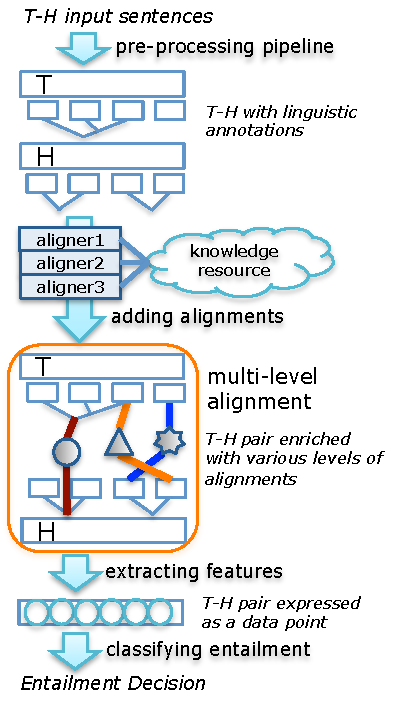
\includegraphics[width=0.9\columnwidth]{figures/figure1.pdf}
  \caption{Dataflow of the proposed approach}
  \label{fig:1}
\end{figure}

The Text (T) and Hypothesis (H) first get pre-processing, such as
POS tagging, lemmatizer, dependency parser and NER. Then, the 
annotated T and H becomes the input for various individual
aligners. Each aligner in the figure can use knowledge resources 
(hence, enrichment step is abstracted within each aligner in
this setup).

The collective alignment data generated by each individual aligner are
stored in one data structure. This is named as {\em Multi-level
  alignments} in the figure. We envision that this representation can
hold different layers of alignments: for example, alignments that
links surface level (tokens), lemma levels, syntactic levels
(e.g. dependency structures), predicate levels, and so on. Also,
analysis results normally not treated as alignment, can be expressed
here as a type of alignment; such as negation analysis result
(e.g. this verb on T is negated on H), or predicate (in-)compatibility
links (e.g. the verb on T express possibility, while the main verb of
H express actuality). 

The next step of the figure is feature extraction. Various features
are extracted from the available alignments (essentially
local-analysis results reported from the aligners), and forms a
feature vector represents the T-H pair. Then, the vector is classified
via a general classifier trained with a training data.   

One notable deviation from conceptual alignment-based architecture
here is that, we intentionally leaving out the step of {\em alignment 
selection}. Alignment selection is a process where the system
finalizes alignments by explicitly assigns a specific portion of T to  
a specific position of H as the one correct alignment. Our choice of
not doing this is closely related to the fact that we envision
multi-level alignments to hold non-traditional alignments which cannot
easily mapped into one single alignment. Getting the global view of
the T-H pair is postponed to the feature extraction steps. Basically,
adding additional (more sophisticated) aligner requires designing
additional (specialized) features.   

The main idea of this TE processing flow is making the layer of
multilevel alignment structure as open as possible for future 
addition of new aligners (here, it is also analyzers). We believe this
can be done by making the data structure for alignments clearly
defined for extensions, and also making the whole algorithm (also code
and implementation) very easy to understand and access.  

% maybe omit --- duplicated in next section 
Thus, implementing this layer is a very important task for the
proposed architecture. For this, we borrowed the data structure from
a TE open-source platform \cite{}. On top of this, we  added {\em
alignment links} as a generic type that can link any linguistic
annotation data within the data type. This enabled us to represent
multi-level alignment layer that can hold any (even future) alignment
analysis outputs.

Naturally, this comes with a cost that each aligner (analyzer)
developer need to learn how to access this common data structure.
We believe this is an acceptable cost, expecially when this data
structure already comes with good representation of multi-lingual
pre-processing pipelines and extensible annotation data
representations. 

% maybe omit --- not many people are interested in SE (software
% engineering) aspects 
One important aspect of the architecture is establishing {\em
orthogonality} \cite{} between aligner (analysis) modules: adding a
new module does not require knowledge of what other modules (aligners)
are doing. This is already true in the pilot implementation, which is
described in the next section. 

\section{Implementation and Evaluation}
\label{sec:impl}
We report a pilot, baseline implementation that tests the potential of 
the proposed architecture. This section first describes the
implementation, then shows the evaluation of the system on two
multi-lingual test set. The implementation, and its source code can 
be accessed from the project homepage \footnote{{URL} anonymized.}.    

\subsection{Pre-processing, knowledge resource, and data
  representation}  
We utilize an open source TE development platform \cite{} as the 
supporting tools for our architecture. The platform provides various   
multilingual pre-processing pipelines, and also knowledge in a
standardized manner for our target languages.
For pre-processing, we have used Maltparser pipelines with TreeTagger
models for all three languages. All knowledge resources (such as
WordNet, VerbOcean, etc) reported in this paper are accessed via the 
platform.    

Another important service that is provided by the platform is the
capability of representing complex data types in a common data
representation. The platform uses UIMA CAS \cite{} as the data
container \cite{}, and defines various annotation types which can be
extended in a coherent manner. This naturally includes linguistic
annotations (such as POS, lemma, parse tree, NER...), but it also
includes the ability to add new meta data type, such as
alignments. This enabled us to define a multilingual multi-level
alignment representation layer, with minimal new data type
definitions. By utilizing those existing modules of a common platform,
we were able to concentrate on the core-algorithm implementations.  

\subsection{The (minimal) aligners}
We used two main aligners for the pilot study. The first aligner is
a generic lexical aligner that works on lemmas via lexical resources,
and the other is a phrase aligner that works on consecutive tokens.  

\paragraph{Lexical aligner} Lexical aligner adds alignment links by
looking up all possible connections between T-H lemmas. If a
relationship is found between two lemmas (one on T and the other on H)
from the given lexical resource, the aligner adds a link between
them. The link has a direction, and has properties of relation name,
and relation strength. Relation name records the type of relation
reported by the lexical resource (such as ``synonym'',
``antonym''). Relation strength is a property that shows the strength
(likelihood) of the relationship, which is often reported by an
automatically built resources such as distributional semantics
tools. The aligner adds all possible links that can be found by the
given lexical resource on the given T-H pair.  

For English, WordNet and VerbOcean were used as the lexical
resources. Italian WordNet was used for Italian, and GermaNet and
German DerivBase \cite{} were used as lexical resources for German. 

\paragraph{Paraphrase aligner} Paraphrase aligner is similar to the
lexical aligner, but what it connects are surface level (tokens),
and it concentrated on more specific resource; the monolingual
paraphrase tables automatically generated by pivot-translation of
Machine Translation tools \cite{}. The alignment links reported by
this aligner has only one relation (paraphrase), but they report
strength of the relation via the translation probability of the
paraphrase. 

In addition to the two aligners, identical lemmas are also aligned
between T-H, without any additional information. In all cases,
aligners report any possible connections they could find, without
regard to existing alignment links.  

Note that the aligners here are minimal, and forms a test-bed, or a
baseline, where additional aligner (analysis) developers can add new
aligners and observe their impacts on TE evaluation. Incorporating
more sophisticated aligners for each language is future work of this
study. Additional aligners such as predicate-compatibility aligner
(for English), and negation aligners (for English and Italian) are
currently in plan.  

\subsection{The (minimal) features} 
We used a set of language independent features in this pilot study. 

The first set is word coverage ratios that measure how much of the
Hypothesis (H) words are covered by local relationship from Text (T)
words. This includes word coverage ratio, and content word coverage
ratio. For the content-word coverage ratio, function words are
filtered based on (language independent) POS classes. The two features 
express general assumption that the more H content covered, the more
likely it is entailment. 

Two other features are Verb coverage, and Proper name coverage
features. Verb-coverage ratio estimates the chance that some
predicate is missed and not covered on Hypothesis. 
Proper name coverage features estimates the chance that the Hypothesis
has a new entity names introduced in H that is not covered by the
components of T. 

Again, the features adopted here can be considered as the base-line
for the approach. Adding new aligners, naturally, requires adding more 
sophisticated features that utilize the added analysis of the new
aligners. We expect that this feature design process is not trivial
and remain to be tested in future work.  

\subsection{Experimental results} 
RTE3 was one of the evaluation workshop for TE community \cite{}. The
evaluation data holds 800 training and 800 testing T-H pairs, and 
later they were translated to both German and Italian. As far as we
know, this is the only RTE evaluation data that is available in
multiple languages with same content. The following table shows the
evaluation result  of the pilot study, marked as {\em proposed},
compared to three other  open-source TE systems that we have tested
with. 

\begin{table}[t!]
\centering
\small
\begin{tabular}{l|ccc}
          &   English   &   German   &   Italian \\
\hline
{\em proposed}&   0.6700      &   0.6450    &  0.6537  \\
BIUTEE        &   0.6700      &     -       &     -    \\
TIE           &   0.652       &   0.6312    &     -    \\ 
EDITS         &   0.6362      &     -       &  0.6262  \\
RTE3 median   &   0.6175      &             &          \\

\end{tabular}
\caption{Evaluation result on RTE3 data set (accuracy).}
\label{table:rte3}
\end{table}

Each of the open source system is configured with their best known
configurations as reported by the developers. The pilot system
supports all three languages, while others supports one (BIUTEE,
English only) or two languages (EDITS, TIE). The pilot system
performed well in all three languages and scored the best among the
tested systems. It ties on the accuracy score with BIUTEE on English,
and it outperforms both EDITS and TIE on English, German and Italian.  

Second task for evaluation is Entailment Graph building. It is an
application task that builds a graph that helps readers to explore
texts in statement levels. Building of the graph requires a TE engine,
and the performance of TE engine is often evaluated with F-1 measure
in this setup. See \cite{} and \cite{} for more information about the
task and data.
The data are from real-world texts of customer interaction domain, and 
they provide large training / test set for TE engine (5300 pairs for
English, 1700 pairs for Italian, etc). Unlike RTE3 data, each data
originated from actual native speakers, and not translated data. Table 
\ref{table:egraph} shows our evaluation results.        

\begin{table}[t!]
\centering
\small
\begin{tabular}{l|ccc}
              &   English    &   Italian   &  German  \\
\hline
{\em proposed}&   0.6915     &   0.6949    &   0.7240  \\
BIUTEE        &   0.7125     &     -       &     -     \\
EDITS         &      -       &   0.6562    &     -     \\
TIE           &      -       &     -       &   0.7241  \\ 
\end{tabular}
\caption{Evaluation result on entailment graph data (f-1 measure)}
% balanced, pure-split data.  
\label{table:egraph}
\end{table}

For this task, we ran two systems for each data. One is our pilot
system, and the other is the best engine reported for the data. The
pilot system beats EDITS in Italian data, and closely follows TIE in
German data, while BIUTEE outperforms the pilot system in English
data.   

The two evaluation results show that the pilot system is already
competing with the state-of-the-art open-source TE engines. The fact 
is even more impressive considering that the pilot system is one
system that works on all three languages. We interpret this result as a
positive sign for the future of the proposed architecture, since the
simple baseline for the approach already competes with complex,
mono-lingual TE systems. 

\section{Conclusion (0.5 page)}
This paper introduced a TE architecture that relies on a layer called
{\em multi-level alignments}. The approach closely follows successful  
alignment-based TE architectures, but differs in the sense that the
proposed method encourages having multiple alignments co-existing in 
one common data structure. The approach suggests using this structure
as the ``firewall'' for all analysis, and making TE engine more open
for future improvements.

We reported a baseline, pilot system of this approach, and evaluated
the performance compared to other open-source TE engines. The pilot
system already competes with the state-of-the-art. The system is
extensible, small and robust, and works with multilingual input out of
the box. It is available as open-source, and can be used by 
anyone who requires a multilingual TE engine. We believe that the 
resulting system is easier to access, modify and extend compared to
other open-source TE engines.

%% \section*{Acknowledgments}

%% Do not number the acknowledgment section.
\bibliographystyle{naaclhlt2015}
\bibliography{sem2015_short}

\end{document}
